\documentclass[12pt, a4paper]{article}
\usepackage[utf8]{inputenc}
\usepackage[IL2]{fontenc}
\usepackage[czech]{babel}
\usepackage{graphicx}
\usepackage[export]{adjustbox}
\usepackage[hidelinks]{hyperref}
\usepackage{url}
\usepackage{breakurl}
\usepackage{float}

\usepackage{listings}
\usepackage{color}

\newcommand{\myparagraph}[1]{\paragraph{#1}\mbox{}\\}

\definecolor{dkgreen}{rgb}{0,0.6,0}
\definecolor{gray}{rgb}{0.5,0.5,0.5}
\definecolor{mauve}{rgb}{0.58,0,0.82}

\lstset{frame=tb,
  language=Java,
  aboveskip=1mm,
  belowskip=1mm,
  showstringspaces=false,
  columns=flexible,
  basicstyle={\small\ttfamily},
  numbers=none,
  numberstyle=\tiny\color{gray},
  keywordstyle=\color{blue},
  commentstyle=\color{dkgreen},
  stringstyle=\color{mauve},
  breaklines=true,
  breakatwhitespace=true,
  tabsize=3
}

\title{\textbf{Dokumentace semestrální práce} \\KIV/WEB}
\author{Jan Čarnogurský}
\begin{document}

\begin{titlepage}
	\newcommand{\HRule}{\rule{\linewidth}{0.3mm}}
	\begin{center}
	
\includegraphics[width=6cm]{img/logo}\\
	\textsc{\LARGE Západočeská univerzita v Plzni}\\[1.5cm]
	\end{center}
	\textsc{\Large Formální jazyky a překladače}\\[0.5cm]
	\textsc{\large KIV/FJP}\\[0.5cm]
	\HRule\\[0.2cm]
	\begin{center}
	{\bfseries \uv{Java} do PL/0}\\[0.5cm]
	\end{center}
	\HRule\\[1.5cm]


	\begin{minipage}{\textwidth}
		\begin{flushleft}
			{\Large Čarnogurský Jan, Vojtěch Danišík\par}
			{\Large A19N0025P, A19N0028P\par}
			{\Large cagy@students.zcu.cz, danisik@students.zcu.cz\par}
		\end{flushleft}
	\end{minipage}
	\vfill\vfill\vfill
	\begin{flushright}
	{\large\today}
	\end{flushright}
	\vfill
\end{titlepage}

\tableofcontents
\thispagestyle{empty}
\clearpage

\newpage
\section{Zadání}
\subsection{Tvorba překladače zvoleného jazyka}
\setcounter{page}{1}

Cílem práce bude vytvoření překladače zvoleného jazyka. Je možné inspirovat se jazykem PL/0, vybrat si podmnožinu nějakého existujícího jazyka nebo si navrhnout jazyk zcela vlastní. Dále je také potřeba zvolit si pro jakou architekturu bude jazyk překládán (doporučeny jsou instrukce PL/0, ale je možné zvolit jakoukoliv instrukční sadu pro kterou budete mít interpret).

\mbox{}\\
\noindent Jazyk musí mít minimálně následující konstrukce:
\begin{itemize}
\item definice celočíselných proměnných
\item definice celočíselných konstant
\item přiřazení
\item základní aritmetiku a logiku (+, -, *, /, AND, OR, negace a závorky, operátory pro porovnání čísel)
\item cyklus (libovolný)
\item jednoduchou podmínku (if bez else)
\item definice podprogramu (procedura, funkce, metoda) a jeho volání
\end{itemize}

\noindent Překladač který bude umět tyto základní věci bude hodnocen deseti body. Další body (alespoň do minimálních 20) je možné získat na základě rozšíření, jsou rozděleny do dvou skupin, jednodušší za jeden bod a složitější za dva až tři body. Další rozšíření je možno doplnit po konzultaci, s ohodnocením podle odhadnuté náročnosti.

\mbox{}\\
\noindent Jednoduché rozšíření (1 bod):
\begin{itemize}
\item každý další typ cyklu (for, do .. while, while .. do, repeat .. unitl, foreach pro pole)
\item else větev
\item datový typ boolean a logické operace s ním
\item datový typ real (s celočíselnými instrukcemi)
\item datový typ string (s operátory pro spojování řětezců)
\item rozvětvená podmínka (switch, case)
\item násobné přiřazení (a = b = c = d = 3;)
\item podmíněné přiřazení / ternární operátor (min = (a < b) ? a : b;)
\item paralelní přiřazení ({a, b, c, d} = {1, 2, 3, 4};)
\item příkazy pro vstup a výstup (read, write - potřebuje vhodné instrukce které bude možné využít)
\end{itemize}


\noindent Složitěší rozšíření (2 body):
\begin{itemize}
\item příkaz GOTO (pozor na vzdálené skoky)
\item datový typ ratio (s celočíselnými instrukcemi)
\item složený datový typ (Record)
\item pole a práce s jeho prvky
\item operátor pro porovnání řetězců
\item parametry předávané hodnotou
\item návratová hodnota podprogramu
\item objekty bez polymorfismu
\item anonymní vnitřní funkce (lambda výrazy)
\end{itemize}


\noindent Rozšíření vyžadující složitější instrukční sadu než má PL/0 (3 body):
\begin{itemize}
\item dynamicky přiřazovaná paměť - práce s ukazateli
\item parametry předávané odkazem
\item objektové konstrukce s polymorfním chováním
\item instanceof operátor
\item anonymní vnitřní funkce (lambda výrazy) které lze předat jako parametr
\item mechanismus zpracování výjimek
\end{itemize}

\subsection{Bodované náležitosti}
Kromě toho že by program měl fungovat se zohledňují i další věci, které mohou pozitivně nebo negativně ovlivnit bodování:
\begin{itemize}
\item testování - tvorba rozumné automatické testovací sady +3 body (pro inspiraci hledejte test suit pro LLVM nebo se podívejte na Plum Hall testy, ale jde skutečně jen o inspiraci, stačí výrazně jednodušší řešení). Užitečné a s tručné povídání na dané téma najdete také tady .
\item Kvalita dokumentace -x bodů až +2 body podle kvality a prohřešků (vynechaná gramatika, nesrozumitelné věty, příliš chyb a překlepů, bitmapové obrázky pro diagramy s kompresními artefakty, ...).
\item Vedení projektu v GITu -x bodů až +2 body podle důslednosti a struktury příspěvků.
\item Kvalita zdrojového textu -x bodů až +2 body podle obecně znýmách pravidel ze ZSWI, PPA a podobně (magická čísla, struktura programu a dekompozice problému, božské třídy a metody, ...)
\end{itemize}

\section{Návrh jazyka}
\subsection{Zvolené konstrukce}
Pro naší semestrální práci jsme zvolili následující konstrukce:
\begin{itemize}
\item minimální konstrukce
\item zbylé cykly (bez foreach)
\item else větev
\item datový typ boolean a logické operace s ním
\item rozvětvená podmínka (switch, case)
\item násobné přiřazení (a = b = c = d = 3;)
\item parametry předávané hodnotou
\item návratová hodnota podprogramu
\end{itemize}

\subsection{Struktura jazyka}
Náš jazyk připomíná Javu, z které vychází. Popis námi zvolené gramatiky je v souboru \texttt{SimpleJava.g4}, který se nachází ve složce se zdrojovými soubory. Pro demonstraci funkčnosti gramatiky jsou v sekci \ref{fig:ukazky} předvedeny všechny možné konstrukce. Tělo programu musí být umístěno ve složených závorkách.

\subsubsection{Omezení jazyka}
\begin{itemize}
\item jazyk používá striktní typování
\item při deklaraci proměnné je vždy nutné nastavit její hodnotu
\item z metody nelze vyskočit dřív než před koncem jejího bloku
\item void metody neobsahují return
\item při rekurzivním volání nelze přistupovat ke globálním proměnným. Viz \ref{fig:volani}
\item iterační proměnná \texttt{for} cyklu nesmí být deklarována
\end{itemize}

\subsubsection{Ukázky jednotlivých konstrukcí}\label{fig:ukazky}
Detailnější ukázky programů jsou uloženy ve složce \textit{testFiles}. Blok programu musí být vždy ve složených závorkách.
\myparagraph{Deklarace proměnných}
\begin{lstlisting}
{
	const int a = 10;
	boolean b = true;
	int d = c = a;
	int a = volaniMetodyNavratovaHodnota(1, false);
}
\end{lstlisting}
\newpage
\myparagraph{Deklarace metod}
\begin{lstlisting}
{
	int function metoda1(int a, boolean b)
	{
		return a + b;
	}

	// pokud je metoda typu void neobsahuje return
	void function metoda2(){}
}
\end{lstlisting}

\myparagraph{Cykly}
\begin{lstlisting}
{
	for(a = 0 ... 10) // odpovida 0 <= 10
	{
		// telo
	}

	while(true)
	{
		// telo
	}

	do
	{
		// telo
	}while(true)

	repeat
	{
		// telo
	}until(false)
}
\end{lstlisting}
\newpage
\myparagraph{If else}
\begin{lstlisting}
{
	if (a < b)
	{
		// telo
	}
	else
	{
		// telo
	}
}
\end{lstlisting}
\myparagraph{Rozvětvená podmínka}
\begin{lstlisting}
{
	switch(cislo) {
		case 1 :
		{
			// telo
		}
		case 2 :
		{
			// telo
		}
		default :
		{
			// telo
		}
	}
}
\end{lstlisting}

\myparagraph{Volání metod}
\begin{lstlisting}
{
	volaniMetody(1, true);

	int a = volaniMetodyNavratovaHodnota(1, false);
}
\end{lstlisting}
\newpage
\section{Implementace}
\subsection{Struktura projektu}
Projekt obsahuje dva hlavní balíky \texttt{generate} a \texttt{compilator}. Balík \texttt{generate} obsahuje třídy vygenerované pomocí \textsf{ANTLR}. Balík \texttt{compilator} obsahuje následující strukturu:
\begin{itemize}
\item \texttt{compilerPart} - balík, který obsahuje třídy pro generování instrukcí
\item \texttt{enums} - balík, obsahuje všechny výčtové typy
\item \texttt{error} - balík s error třídami
\item \texttt{object} - balík se společnými objekty
\item \texttt{visitor} - balík, který obsahuje visitory pro průchod derivačního stromu
\item \texttt{Compilator} - třída, která obsluhuje proces aplikace
\item \texttt{ErrorHandler} - třída pro obsluhu chyb při generování instrukcí
\item \texttt{InstructionGenerator} - třída pro spuštění generování instrukcí
\item \texttt{LexerParserErrorListener} - třída pro obsluhu chyb při parsování vstupního souboru
\end{itemize}

\subsection{Princip funkčnosti}
\noindent Zpracování je rozděleno do několika kroků. Průběh zpracování je znázorněn na obrázku \ref{fig:zpracovani}. O průběh zpracování se stará třída \texttt{Compilator}, která jednotlivé bloky spouští. Třída \texttt{Compilator} je volána z třídy \texttt{Main}, a jako parametry jsou předány cesty k vstupnímu a výstupnímu souboru. Kód je generován na dva průchody. Prvním průchodem se uloží derivační strom do paměti a druhým průchodem se z uložených struktur v paměti vygenerují instrukce.

\begin{figure}[!h]
  \centering
  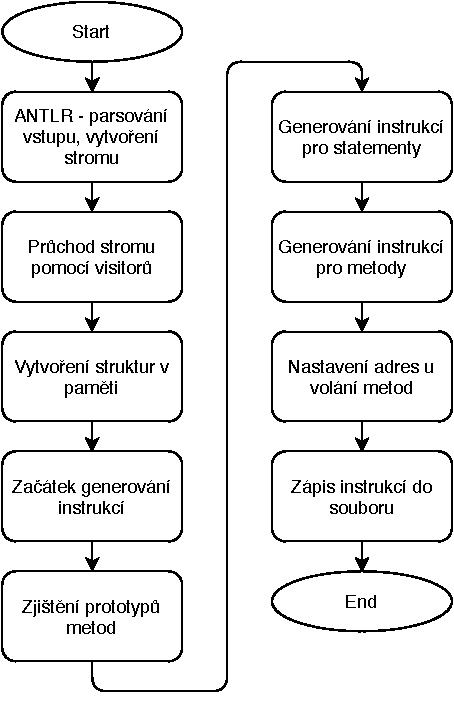
\includegraphics[scale=0.8]{img/diagram.pdf}
  \caption{Průběh zpracování}
  \label{fig:zpracovani}
\end{figure}
\newpage
\subsubsection{Parsování vstupního souboru}
\noindent Parsování vstupu, vytvoření derivačního stromu, a jeho zpracování je řešeno pomocí \textsf{ANTLR}. Gramatika je popsána v souboru \texttt{SimpleJava.g4}. Soubory vytvořené pomocí \textsf{ANTLR} jsou vygenerovány do balíku \texttt{generate}.

\subsubsection{Průchod stromu}
\noindent Průchod stromu je řešen pomocí \texttt{visitorů}. Jednotlivé \texttt{visitory} jsou uloženy v balíku \texttt{compilator/visitor}. \texttt{Visitory} jsou rozděleny do tříd tak, aby odpovídaly hlavním uzlům v derivačním stromu. \texttt{Visitory} slouží k průchodu stromu, a k jeho následnému uložení do paměti.

\subsubsection{Struktury v paměti}
\noindent Struktury v paměti slouží pro uložení derivačního stromu do paměti, aby s ním bylo možné dále pracovat. Názvy struktur odpovídají hlavním položkám v gramatice. Výsledkem průchodu je objekt \texttt{Program}, který představuje kořen derivačního stromu a obsahuje odkazy na další objekty (uzly), které obsahují další odkazy.

\subsubsection{Začátek generování instrukcí}
\noindent V této částí je program přepnut do zpracování uložené struktury v paměti. Je zavolána třída \texttt{InstructionGenerator} a je jí předán objekt \texttt{Program}. Výsledkem generování instrukcí je list vygenerovaných instrukcí.

\subsubsection{Prototypy metod}
\noindent Před samotným generováním instrukcí je nejprve nutné zjistit prototypy metod (hlavičky metod), aby při generování volání metod bylo možné určit, jestli metoda má návratovou hodnotu, popřípadě jakého je typu. Prototypy metod nepracují s parametry.

\subsubsection{Generování instrukcí}
\noindent Pro generování instrukcí je připraveno několik tříd, kde každá zpracovává různě námi uložené struktury:
\begin{itemize}
	\item \texttt{BaseCompiler} - abstraktní třída od které jsou další třídy odděděny. Obsahuje společné proměnné
	\item \texttt{ProgramCompiler} - zpracovává objekt \texttt{Program}
	\item \texttt{BlockCompiler} - zpracovává objekt \texttt{Block}
	\item \texttt{BlockStatementCompiler} - zpracovává objekt \texttt{BlockStatement}, ve kterém jsou uložena veškerá těla metod. Uvnitř tohoto kompileru jsou volány subpřekladače (\texttt{ExpressionCompiler, MethodCallCompiler, \newline Methodompiler}), dle potřeby
	\item \texttt{ExpressionCompiler} - zpracovává objekt \texttt{Expression}, který představuje veškeré výrazy
	\item \texttt{MethodCallCompiler} - zpracovává objekt \texttt{MethodCall}, který představuje volání metod
	\item \texttt{MethodCompiler} - zpracovává objekt \texttt{Metod}, který představuje deklaraci metod
\end{itemize}

Generování je rozděleno do dvou kroků. Prvním krokem je vygenerování instrukcí pro hlavní tělo programu, druhým krokem je vygenerování instrukcí pro metody. To způsobí, že začátek programu je vždy ve výsledných instrukcích uložen na adrese jedna a metody jsou uloženy na konci.

\subsubsection{Nastavení adres u volání metod}
\noindent Tím, že je umožněno, aby metody byly vytvořeny až po jejich zavolání, je nutné u instrukcí pro volání metod zpětně nastavit adresu, na které se volaná metoda nachází. Tyto instrukce jsou uloženy s adresou \uv{-1} navíc je to objektu představující instrukci uložen objekt \texttt{MethodCall}.

V cyklu se projdou veškeré instrukce a pokud se jedná o instrukci \texttt{CALL}, je z objektu instrukce získán objekt \texttt{MethodCall}. Zkontroluje se, zda název metody uložený v \texttt{MethodCall} existuje v tabulce symbolů, dále se zkontrolují zda sedí počet a typ parametrů. Pokud není cokoliv splněno je vyhozena chyba a program je ukončen. Pokud je vše splněno, je instrukci \texttt{CALL} změněna adresa podle tabulky symbolů.

\subsubsection{Nastavení levelů u volání metod} \label{fig:nastaveni}
\noindent Při volání metody v metodě je nutné u instrukce \texttt{CALL} zvýšit její level, aby	když volaná metoda chtěla přístup ke globální proměnné, tak aby se správně posunula	báze.

V cyklu se prochází vygenerované instrukce. Pokud se najde instruce \texttt{RET}, cyklus končí. Pokud se najde instrukce \texttt{CALL}, je iterovací proměnná změněna na adresu instrukce \texttt{CALL}, instrukce se označí jako aktualizovaná a cyklus se opakuje. Pokud se nalezne další instukce \texttt{CALL} v těle volané metody před instrukcí \texttt{RET}, je instrukci uložen předchozí level zvýšen o jedničku, provede se změna iterační hodnoty proměnné a cyklus se opakuje. Metoda pro opravu levelů se nachází v \texttt{BlockStatementCompiler::updateCallLevel()}.

Tato implementace nese jistá omezení popsaná v kapitole \ref{fig:volani}.

\subsubsection{Zápis instrukcí do souboru}
Instrukce se zapíšou do souboru, který byl zadán jako vstupní parametr. V cyklu se projde list instrukcí, který vrátil objekt \texttt{InstructionGenerator}. Pokud výstupní soubor již existuje, je vždy přepsán novými instrukcemi.

\subsection{Viditelnost proměnných}
\noindent Proměnné nadefinované v hlavním těle programu jsou viditelné v celém kódu (jsou celou dobu držené v tabulce symbolů) a je pro ně zvýšen obsah zásobníku. Pro proměnné nadefinované mimo hlavní blok programu (těla metod, těla smyček, ...), je v momentě vykonávání bloku zvýšen obsah zásobníku, a jsou zahrnuty do tabulky symbolů. Po skončení bloku jsou proměnné odstraněny z tabulky symbolů, a je snížen vrchol zásobníku o jejich počet. Tím je zajištěno, že nejsou dále viditelné.

\subsection{Volání metod s parametry}
\noindent Volání metod je řešeno v \texttt{MethodCall}. Pokud má metoda parametry, které je nutné předat, jsou před instrukcí \texttt{CALL} na vrchol zásobníku přidány hodnoty parametrů. V metodě se zvýší vrchol zásobníku o počet parametrů +3 co představuje defaultní velikost metody. Parametry metody jsou získány pomocí instrukce \texttt{LOD} se zápornou hodnotou. Záporná hodnota odpovídá počtu parametrů. Následně se instrukce \texttt{LOD} volá znovu se zápornou hodnotou změnšenou o jedna. To se opakuje dokud se nenačtou všechny parametry. Načtené hodnoty se průběžně ukládají do tabulky symbolů, aby s nimi bylo možné v metodě dále pracovat. Po návratu z metody je ještě nutné předané parametry odstranit z vrcholu zásobníku. Provede se instrukce \texttt{STO} s hodnotou -1, tolikrát, kolik bylo předáno parametrů.

\subsection{Metoda s návratovou hodnotou}
\noindent Volání metody je řešeno v \texttt{MethodCall}. Pokud má metoda návratovou hodnotu, je před instrukcí \texttt{CALL} zvýšen obsah zásobníku o jedna. Výsledek, který metoda vrací je umístěn za klíčovým slovem \uv{return}. Po vyhodnocení výsledku je výsledek uložen na adresu počet proměnných +1. Tato adresa odpovídá místu, které se vytvořilo na vrcholu zásobníku jeho zvětšením.
\subsection{Error kódy}
\noindent Program pracuje se svými chybovými kódy. Chyby jsou spravovány pomocí třídy \texttt{ErrorHandler}, která se stará o vypsání chyby a ukončení programu s příslušným kódem. Níže jsou popsány chybové kódy s jejich popisem.

\begin{table}[!h]
\centering
\resizebox{\textwidth}{!}{%
\begin{tabular}{|c|c|}
\hline
Kód & Popis                                                                                             \\ \hline
1   & Proměnná, kterou se snažíte přiřadit neexistuje.                                                   \\ \hline
2   & Pokoušíte se přepsat hodnotu u konstanty.                                                          \\ \hline
3   & Při volání metody nesedí počet parametrů.                                                          \\ \hline
4   & Metoda s tímto jménem již existuje.                                                                \\ \hline
5   & Metoda, kterou se snažíte zavolat neexistuje.                                                      \\ \hline
6   & Výsledek výrazu nesedí s očekávaným výsledkem (např. přiřazení matematického výrazu do logického). \\ \hline
7   & Návratový typ metody nesedí s proměnnou, do které se přiřazuje.                                    \\ \hline
8   & Není možné kombinovat logické a matematické výrazy dohromady (např. true + 10).                    \\ \hline
9   & Snaha přiřadit proměnné typu INT hodnotu BOOLEAN a naopak.                                         \\ \hline
10  & Switch nemůže obsahovat více defaultních bloků.                                                    \\ \hline
11  & Proměnná s tímto názvem již je deklarována.                                                        \\ \hline
12  & Snaha pracovat s proměnnou, která neexistuje.                                                      \\ \hline
13  & Při zavolání metody typu void ve výrazu.                                                           \\ \hline
14  & Typy parametrů metody a typy parametrů ve volání se neshodují.                                     \\ \hline
15  & Vstupní soubor neexistuje.                                                                         \\ \hline
16  & Chyba při parsování souboru ANTLR.                                                                 \\ \hline
17  & Neznámá chyba (i když je program otestovaný, může se stát, že se objeví neočekávaná Chyba).										  									                                                                \\ \hline
18  & Chybné spuštění aplikace, nesedí parametry.                                                        \\ \hline
18  & Chybná cesta k výstupnímu souboru.                                                        \\ \hline
\end{tabular}%
}
\end{table}
\newpage
\section{Testování}
\noindent Pro překlad nebyly vytvořeny žádné automatické testy. Testy, které jsme prováděli byly všechny manuální. Všechny námi vytvořené testovací scénáře jsou uloženy ve složce \textit{testFiles}. Pro každý testovací scénář existuje i soubor s výslednými instrukcemi.

\section{Uživatelská dokumentace}
\noindent Pro překlad je nutné mít nainstalovaný \textsf{Maven}. Překlad projektu se provede spuštěním příkazu:
\begin{itemize}
	\item mvn clean install
\end{itemize}

\noindent Pozor, \textsf{Maven} vytvoří dva jar soubory. Aby bylo možné program spustit je nutné pracovat se souborem, který má v názvu \uv{-jar-with-dependencies}.

\mbox{}\\
\noindent Pro spuštění je nutné mít nainstalovanou \textsf{Javu}, program se spouští příkazem:

\begin{itemize}
	\item java -jar \textless nazev JAR \textgreater.jar \textless vstupní soubor \textgreater \textvisiblespace \textless výstupní soubor \textgreater
\end{itemize}

\noindent Pro demonstraci je vytvořen soubor, který provede ukázkové spuštění.
\begin{itemize}
  \item Linux : ./run.sh
  \item Windows : run.bat
\end{itemize}

\mbox{}\\
\noindent V připadě, že nepůjde skript na linuxu spustit je nutné nastavit práva:
\begin{itemize}
\item chmod +x run.bat
\end{itemize}

\noindent Při špatném spuštění, je uživateli vypsána hláška s postupem, jak se program spouští.


\section{Závěr}
\subsection{Omezení při volání metod} \label{fig:volani}
\noindent Při vývoji byl zjištěn problém, který se nám nepodařilo lépe vyřešit. Problém nastává při úpravě levelu u instrukce \texttt{CALL} (viz \ref{fig:volani}) a projevuje se nemožností přistoupit ke globální proměnné ve dvou případech.

Prvním případem, kdy není možné přistoupit ke globální proměnné, je při rekurzivním volání metody. Algoritmus, který je popsán v sekci \ref{fig:volani} způsoboval zacyklení, bylo tedy nutné ošetřit to, že pokud instrukce \texttt{CALL} volá stejnou adresu jako předešlá instrukce \texttt{CALL}, tak aby algoritmus skončil. Tím ale přestane fungovat přístup ke globální proměnné, protože nejsme schopni posunout správně bázi. Celkový výsledek metody je ale vyhodnocen správně. Testováno přes rekurzivní výpočet Fibonacciho čísla. Testovací scénář je uložen v souboru \textit{testFiles/complex/fibonacci.txt}.

Druhým případem, kdy není možné přistoupit ke globální proměnné je znázorněn na obrázku \ref{fig:metody}. Metoda \textsf{A} volá \textsf{B}, \textsf{B} volá \textsf{C}, \textsf{C} volá \textsf{D}, v tomto případě, by přístup ke globální proměnné fungoval správně. Problém ale nastává v momentě, když bude metoda E volat metodu \textsf{C}, která volá \textsf{D}, protože v metodě \textsf{C} je už z prvního volání nastaven posun báze. To způsobí, že nedojde k aktualizaci levelu báze a přistup ke globální proměnné bude fungovat jen v  případě volání z \textsf{A} a v případě volání z \textsf{E} to bude přistupovat na špatnou adresu. To že se neprovede aktualizace je způsobeno identifikátorem, který označuje volání za již aktualizované. I kdyby tato značka nebyla nastavena, způsobilo by to to, že by se level upravil a potom by nefungovalo volání z metody \textsf{A} a fungovalo z metody \textsf{E}

\begin{figure}[!h]
  \centering
  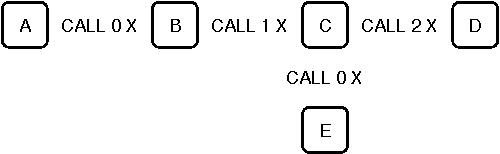
\includegraphics[]{img/metody.pdf}
  \caption{Graf volání metod}
  \label{fig:metody}
\end{figure}

Je možné, že tento nedostatek je způsoben špatným návrhem, ale i teď s odstupem času nás nenapadá, jak by bylo možné tuto chybu odstranit. Bylo by nejspíše nutné pokud jeden z těchto dvou případů nastane vytvořit kopii instrukcí pro metodu, u které by se upravil akorát level, to by ale způsobilo to, že by byly instrukce pro metodu uloženy v instrukcích dvakrát. Zároveň by to neřešilo problém s rekurzí.

\subsection{Zhodnocení výsledků}
I přes výše zmíněný nedostatek se nám podařilo vytvořit překladač, který dokáže náš vytvořený jazyk převést do instrukční sady \textsf{PL/0}. Pro testování bylo vytvořeno několik scénářů, které demonstrují, že si kompilátor dokáže poradit s jednoduššími, ale i se složitějšími konstrukcemi jako je rekurzivní volání.

Semetrální práce byla vedena na adrese \href{https://github.com/danisik/FJP}{https://github.com/danisik/FJP}.

\end{document}
